\documentclass[a4paper, 12pt, twoside]{article}
\usepackage[utf8]{inputenc}		% LaTeX, comprend les accents !
\usepackage[T1]{fontenc}		
\usepackage[francais]{babel}
\usepackage{lmodern}
\usepackage{ae,aecompl}
\usepackage[top=2.5cm, bottom=2cm, 
			left=3cm, right=2.5cm,
			headheight=15pt]{geometry}
\usepackage{graphicx}
\usepackage{eso-pic}	% Nécessaire pour mettre des images en arrière plan
\usepackage{array} 
\usepackage{hyperref}
\input{pagedegarde}


\title{Nebula}
\entreprise{Le nom de votre entreprise}
\datedebut{25 mars 2026}
\datefin{23 mai 2026}



\membrea{Massoud Zaina 44005097}
\membreb{Icheboudene Ilyana 45011072 }
\membrec{Ait-boukhima Dunia 45004863}
\membred{Baghadi Yasmine 45012138} 
\membree{\\[0.5cm] \textbf{Dépôt Github :} \url{https://github.com/yasminebaghdadi/Projet-info}}



\begin{document}
\pagedegarde
\section*{Remerciements}
Nous souhaitons remercier toutes les personnes qui nous ont aidés pendant la réalisation de ce projet (nous même et chat gpt).
Et surtout un grand merci à notre professeur, François Delbot, pour ses cours, sa patience et ses explications. Grâce à son aide et à son accompagnement, nous avons beaucoup appris et nous avons pu avancer dans de bonnes conditions. 

\newpage

\tableofcontents
\newpage

\section{Introduction}
Le saviez-vous ? On oublie environ 95 pour cent de nos rêves quelques minutes après le réveil.
Chaque nuit, notre imagination déborde et prend le contrôle, laissant derrière elle des histoires plus farfelues les unes que les autres.
C’est pour cela que nous avons créé Nebula, un espace où chacun peut capturer ses rêves avant qu’ils ne s’effacent, les partager avec d’autres rêveurs et surtout obtenir une interprétation grâce à notre IA spécialisée dans les rêves.
Qu’ils soient profonds, lucides ou même inexplicables, chaque rêve révèle une émotion, une peur profonde ou est simplement le fruit votre imagination. Il est donc très interessant de les mettre en perspective.
Parce qu'un rêve oublié est une histoire perdue...
\begin{figure}[h]
\centering

\includegraphics{star.png}
\caption{Logo Nebula}
\label{Tux}
\end{figure}



\section{Environnement de travail}
Pour ce projet, nous avons utilisé l’IDE Visual Studio Code, qui permet d’ouvrir
tous les types de fichiers de manière simultanée : HTML, CSS, Python...
Nous avons également utilisé la plateforme Github pour partager notre code.

\section{Description du projet et objectifs}
 

	\subsection{Description du projet}
Notre idée etait de réaliser un site internet interactif consacré aux rêves et a leur interpretation grâce a l'intelligence artificielle l'utilisateur doit d'abord créer un compte avec son adresse mail et un mot de passe, une fois dans le site il arrive directement sur le "feed d'actualité" ou il aura la possibilité d'écrire un nouveau rêve qui sera directement interpréter par l'intelligence artificielle. L'utilisateur peut ensuite décider de garder son rêve privé ou bien de le publier. Il peut aussi consulter les rêves des autres utilisateurs, commenter, liker les publications. 

    
	\subsection{Objectifs}
L'objectif principal de notre projet était de créer un site web permettant aux utilisateurs de raconter leurs rêves et d'obtenir une interprétation par IA. Au-delà de cela nous voulions surtout créer un espace d'échange et de reflexion autour des rêves et des émotions. Les rêves occupent une place importante dans la vie de nombreuses personnes. Ils peuvent refléter des émotions, des peurs, des souvenirs, du stress ou encore des envies inconscientes. À travers ce projet, nous voulions offrir aux utilisateurs un espace où ils pourraient s’exprimer librement, raconter leurs expériences personnelles et essayer de mieux comprendre leurs émotions grâce aux interprétations proposées par l’intelligence artificielle mais également ceux des autres utilisateurs via l'espace commentaire. Nous avons donc essayer de faire un site à la fois personelle et communautaire. Le but était de montrer que certaines personnes peuvent partager les mêmes émotions, les mêmes inquiétudes ou les mêmes expériences à travers leurs rêves ou tout simplement partager leurs avis et discuter librement autour de ce sujet passionant. Enfin, et surtout, nous avions comme but d'ameliorer nos compétences en programation à travers ce projet et de découvrir de nouveaux aspects de l'informatique.

\section{Bibliothèques, Outils et technologies}
Parmi les outils qui nous ont le plus aidés, ChatGPT Plus a eu une place très importante dans le projet. Il nous a accompagné dans la création du code, dans le développement des fonctionnalités et dans la résolution de certains problèmes techniques. Cependant, nous avons rapidement compris que l’intelligence artificielle ne faisait pas tout automatiquement. Pour obtenir un résultat précis, il fallait savoir bien la guider et expliquer clairement ce que nous voulions réaliser. Plus nos demandes étaient détaillées, plus les réponses obtenues étaient adaptées à notre projet. Cette expérience nous a permis de découvrir à quel point l’intelligence artificielle peut être un outil puissant dans le développement informatique, tout en montrant qu’il reste nécessaire de comprendre le code et le fonctionnement du projet pour pouvoir l’utiliser 

 Pour le développement du site, nous avons utilisé Python 3 car c'est a la fois un langage simple et efficace, il nous a permis de mieux comprendre le fonctionnement des différentes fonctionnalités du site.



\begin{figure}[!ht]
\centering
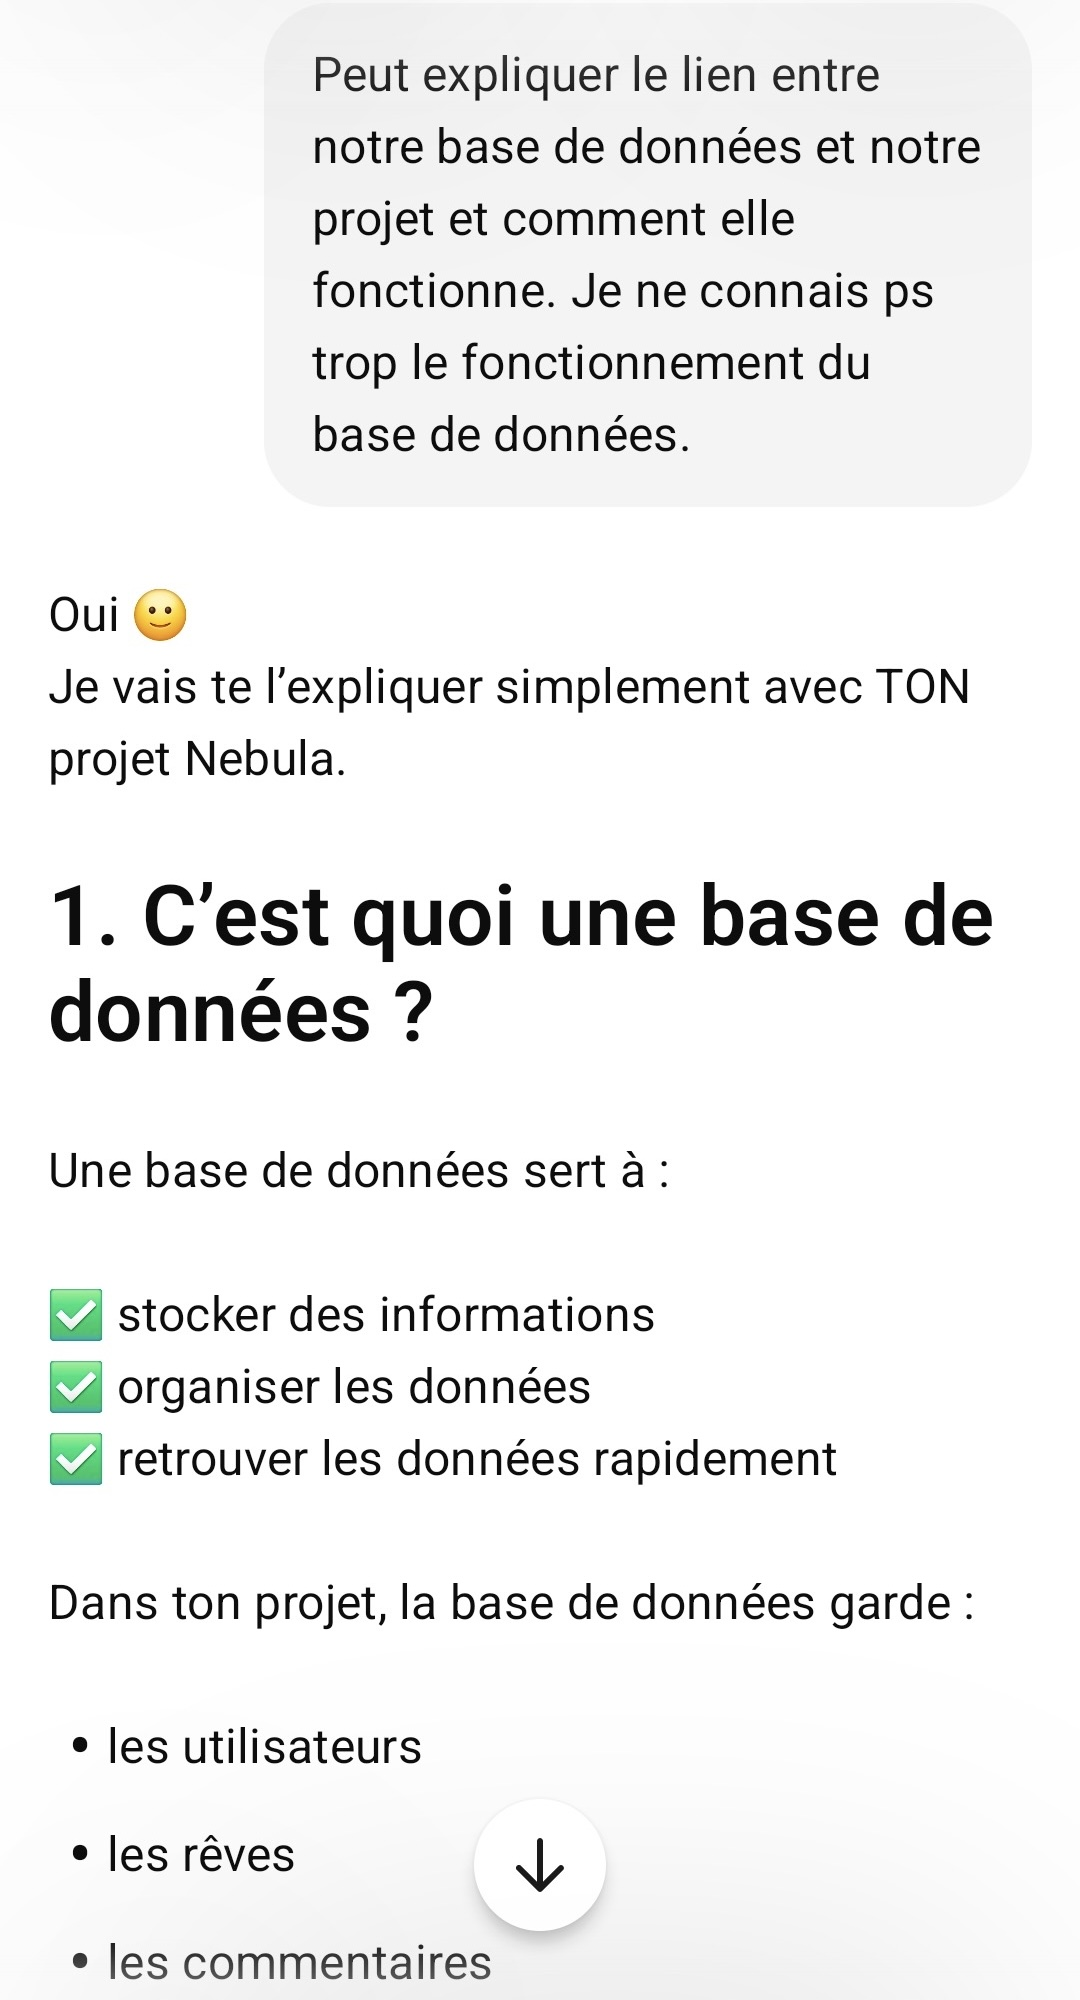
\includegraphics[width=0.5\textwidth]{DB}
\caption{Discussion avec Chatgpt}
\label{fig:structure}
\end{figure}


\newpage




Le projet utilise une base de données locale SQLite appelée dreams.db.
Cette base de données est stockée directement dans le projet sous forme d’un fichier local.Le choix d’une base de données locale a été fait car SQLite est simple à utiliser avec Flask et adapté à un projet web léger sans serveur distant.

nous avions beaucoup de doutes sur le fonctionnement de la base de données donc pour eviter les problèmes de dernière minute nous avons aussi crée une version du projet utilisant des fichiers JSON pour stocker nos données, on l'aurait utiliser comme backup.





Flask est une bibliothèque permettant de créer un site web avec Python. Elle fonctionne avec un système de routes reliées aux pages HTML, ce qui permet d’organiser le site et de gérer les différentes actions des utilisateurs. Lorsque nous exécutions le fichier principal du projet avec la commande python app.py, cela lançait un serveur local permettant d’ouvrir le site directement dans le navigateur via une adresse HTTP. \\




\begin{figure}[h]
\centering
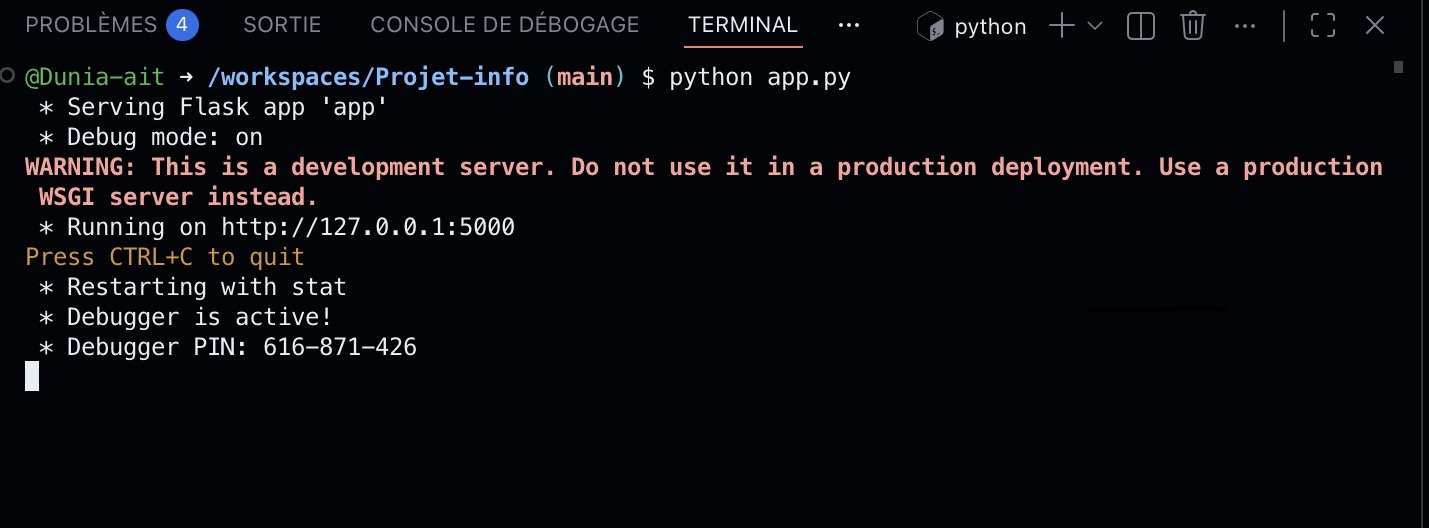
\includegraphics[width=\textwidth]{Terminal}
\caption{Terminal du code}
\label{Tux}
\end{figure}



\newpage
Le développement du projet a été réalisé sur Visual Studio Code (VS Code), qui nous a permis d’écrire, modifier et organiser le code plus facilement. Comme nous travaillions en groupe, nous avons également utilisé GitHub afin de partager le projet, sauvegarder les différentes versions du code et travailler ensemble de manière plus efficace. 

\begin{figure}[h]
\centering
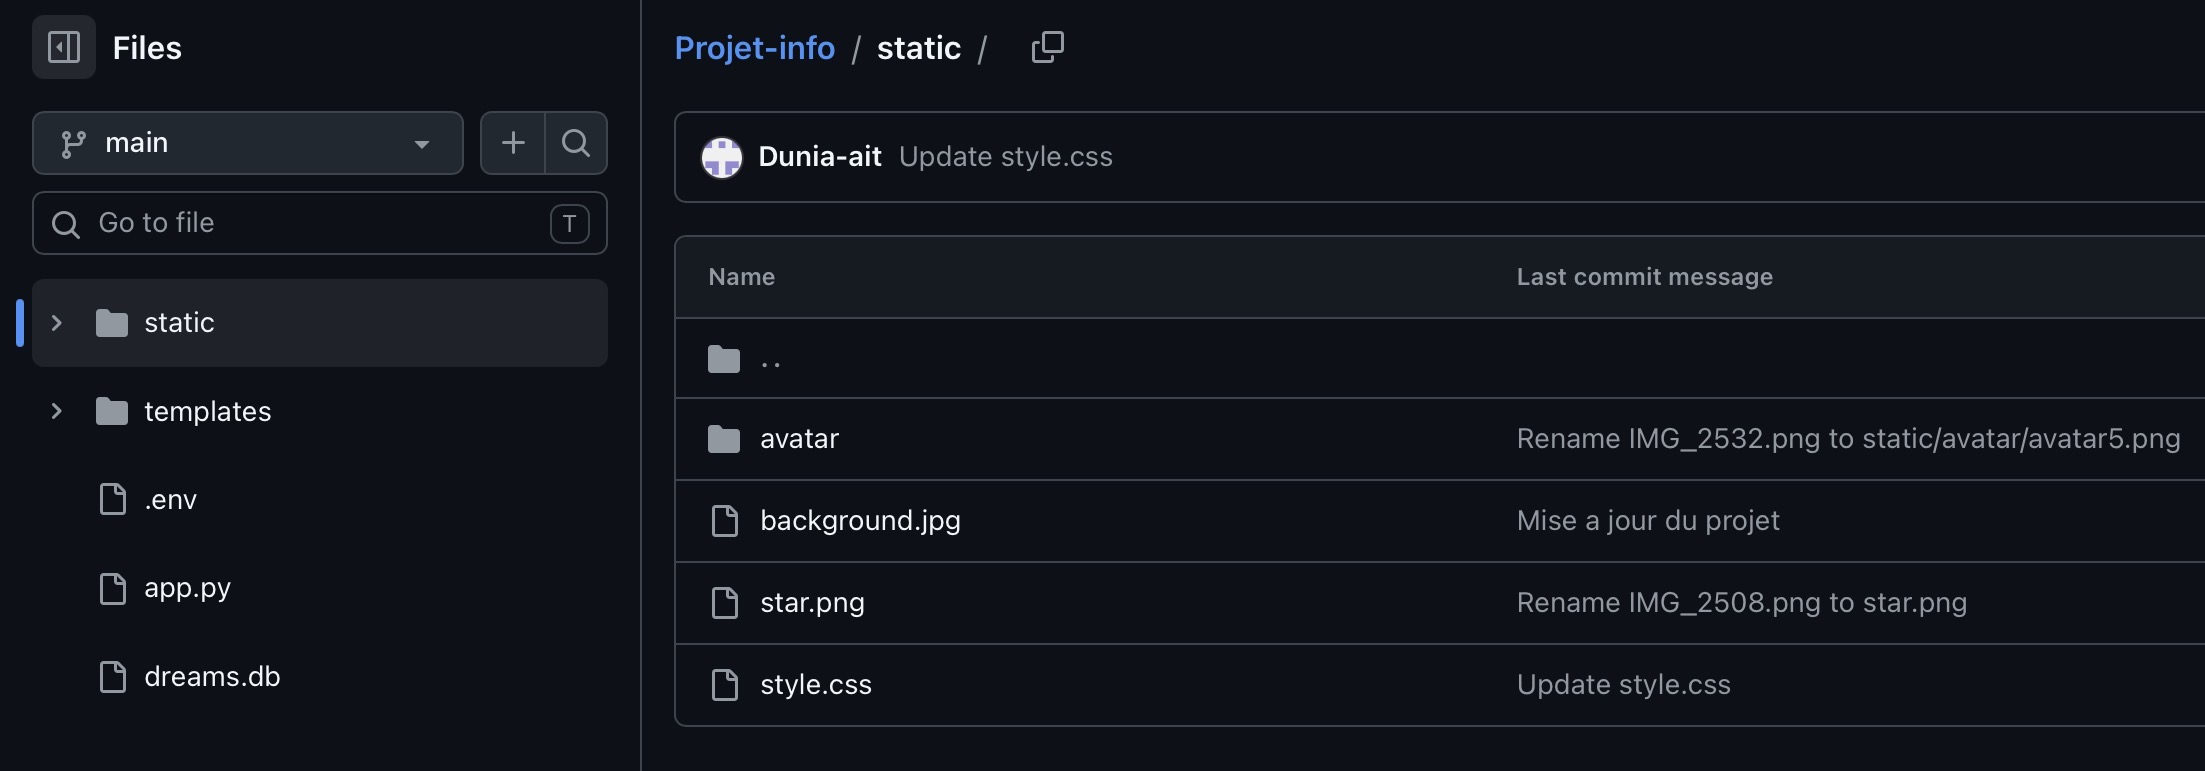
\includegraphics[width=\textwidth]{github}
\caption{Github du groupe}
\label{Tux}
\end{figure}


De plus, nous avons mis une IA sur le site grâce à une clé API gratuite (GROQ API KEY) que nous avons trouver sur : console.groq.com, nous avons du faire appel aux deux bibliotheque : "dotenv" et "groq" pour son utilisation. \\

\begin{figure}[h]
\centering
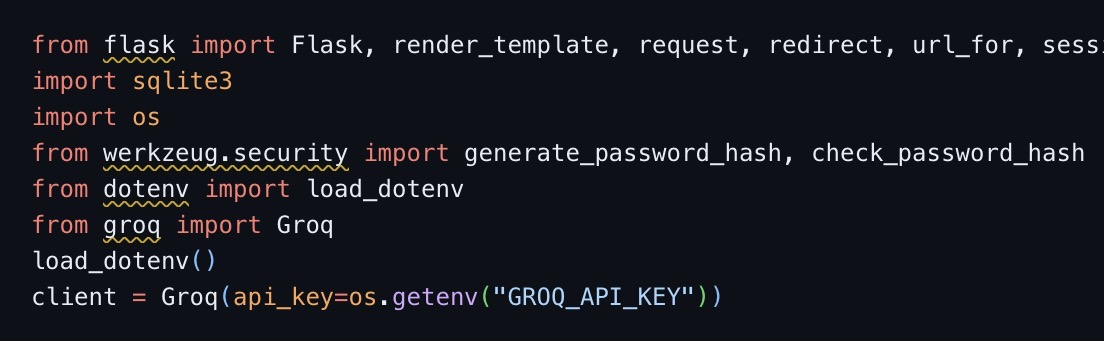
\includegraphics[width=\textwidth]{Bbl}
\caption{Bibliothèques importées}
\label{fig:bibliotheques}
\end{figure}


\newpage

\section{Travail réalisé}

Voici la structure du site :

\begin{figure}[!ht]
\centering
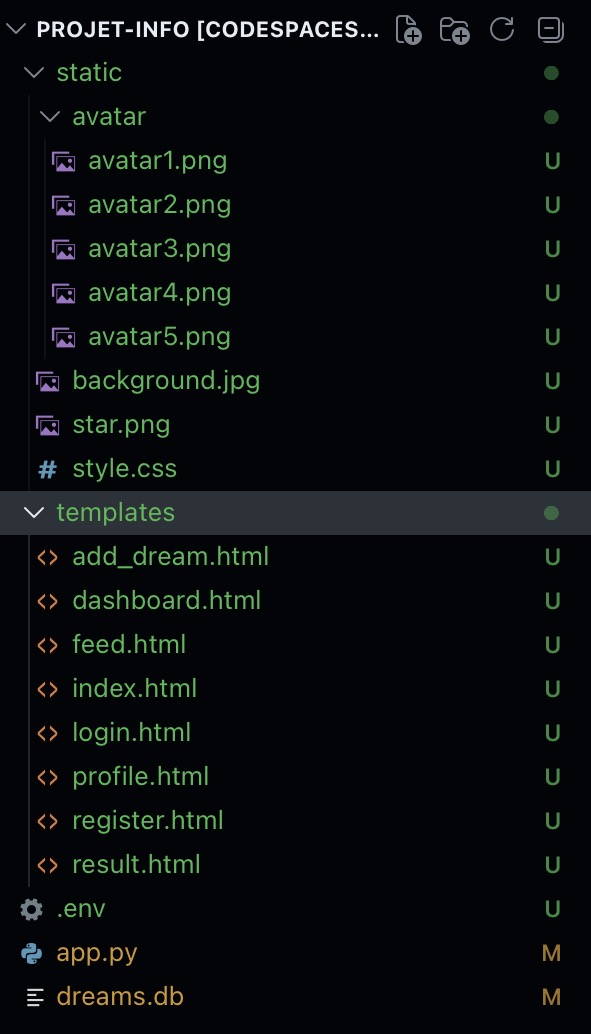
\includegraphics[width=0.5\textwidth]{Struct}
\caption{Structure du site}
\label{fig:structure}
\end{figure}

Lègende : \\
app.py : Fichier principal contenant toutes les routes Flask
Dossier templates : tous les fichiers d’interface HTML (tableau de bord, pages de connexion, profil...) \\
Dossier static : Logo et fichier CSS\\
Dossier avatar : photos de profil proposés\\
Le site correspond dans la majorité à nos attentes en termes de fonctionnalités.
Parmi les fonctionnalités prévues et réalisées :\\
- Un feed public (ou fil d'actualité) avec les rêves publiés et leurs interprétations ainsi qu'un espace commentaire et la possibilité de liker le rêve\\
- Un profil avec tous les rêves ecrient (privé ou public) et un compteur de rêve ou cauchemar \\
- Une création de compte pour permettre une identification et ne pas perdre tous les rêves entrés\\


Voici un exemple d'interprétation de rêve faite par notre intelligence artificielle Groq :
\begin{figure}[!ht]
\centering
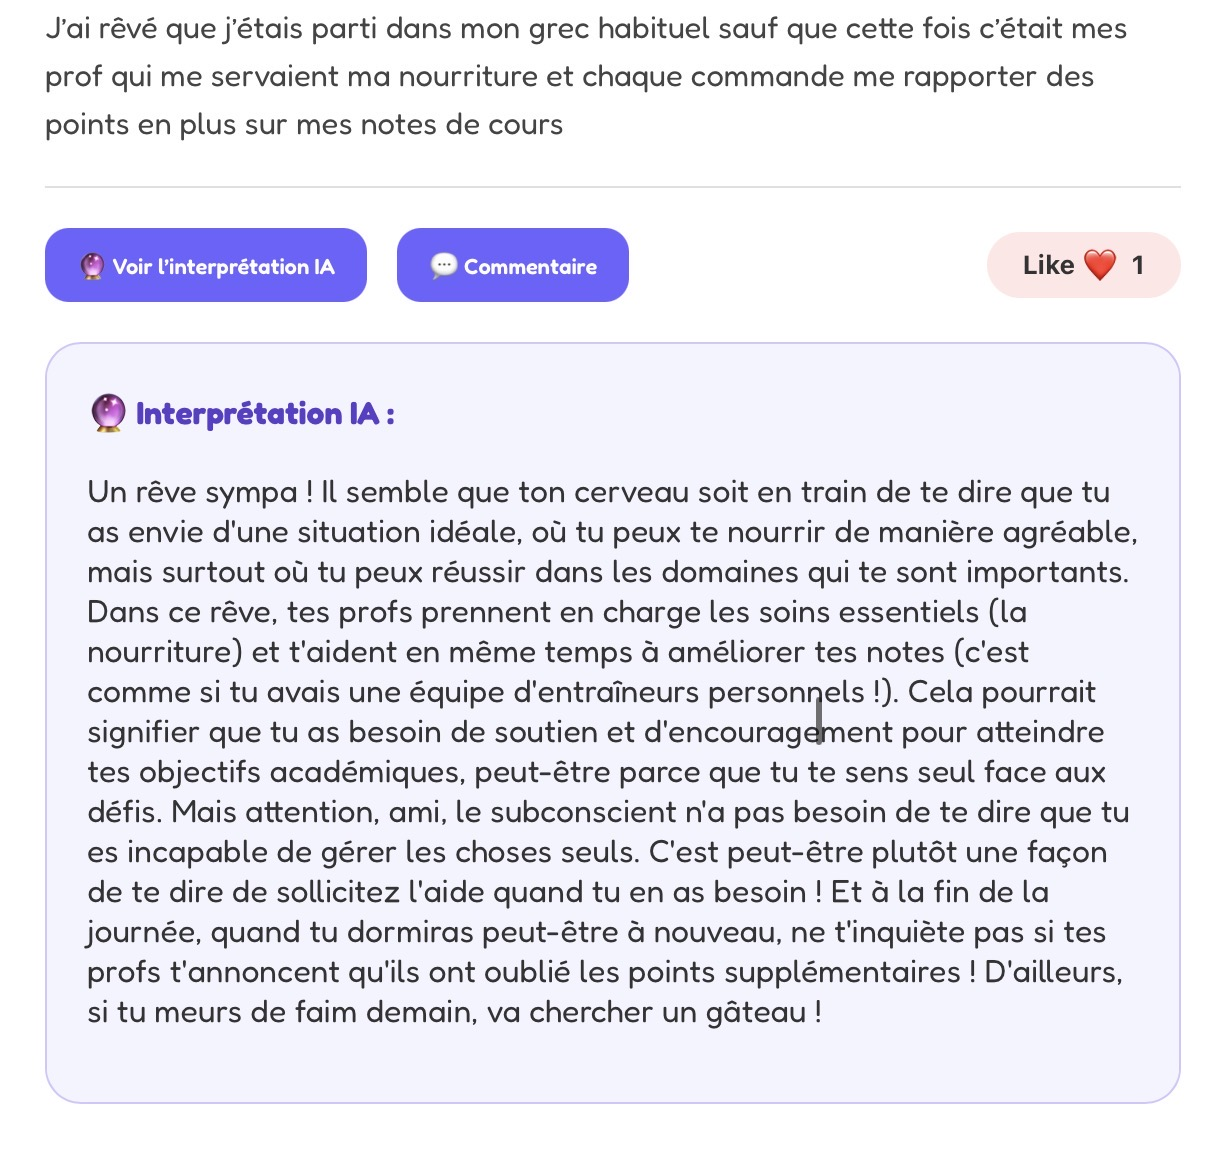
\includegraphics[width=0.5\textwidth]{IA}
\caption{Interprétation par IA}
\label{fig:structure}
\end{figure}


Pour qu'elle interprète de la manière dont on le souhaite nous avons du lui donner certaines instructions :
\begin{figure}[!ht]
\centering
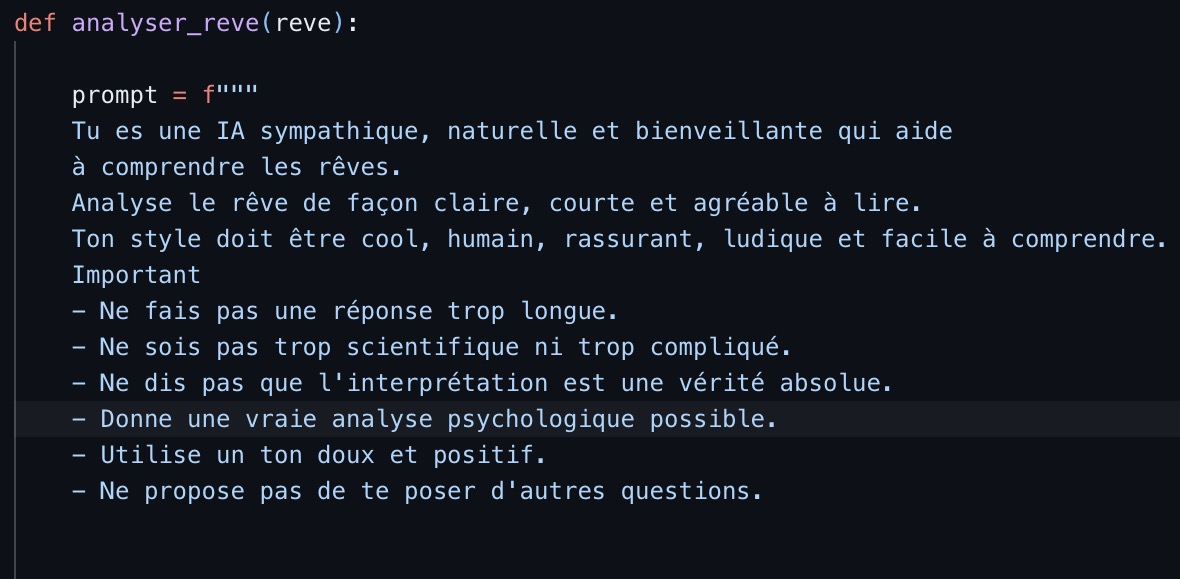
\includegraphics[width=0.5\textwidth]{com}
\caption{Commande IA}
\label{fig:structure}
\end{figure}


En revanche, certaines n’ont pas été à notre portée. Nous n'avons pas pu faire en sorte que l'IA présente dans le site fasse des liens entre les rêves des utilisateurs (similarités, rêve en commun...)
La fonctionalité la plus importante que nous avons pas pu mettre en place est la représentation graphique en 3D des récits qui demandait des ressources énormes sachant que le monde des rêves est très abstrait nous avions peur que l'IA parte dans des interprétations incompréhensibles. \\

Répartition des tâches : une personne était chargée de l’intégration de l’IA et de son bon fonctionnement, une autre s’occupait de l’interface, une autre du profil utilisateur, et une dernière mettait en place les fonctionnalités liées aux interactions (commentaires, likes, etc.). Le compte rendu a été réalisé collectivement par toute l’équipe.

\section{Difficultés rencontrées}





Nous avons rencontré des difficultés lors de l’intégration de l’intelligence artificielle dans le site. Au début, il était compliqué de réussir à installer correctement l’IA et à la connecter au fonctionnement du projet. Une fois cette étape réussie, le plus difficile était surtout de la configurer pour qu’elle interprète les rêves de la manière que nous souhaitions.
En effet, les premières réponses générées étaient parfois trop simples, incohérentes ou ne correspondaient pas vraiment à l’ambiance que nous voulions donner au site. Nous avons donc dû faire plusieurs tests et modifier de nombreuses consignes afin d’obtenir des interprétations plus réalistes, plus humaines et davantage basées sur les émotions et le subconscient.
Nous avons également rencontré beaucoup de problèmes liés à l’indentation du code. Lorsque nous demandions à ChatGPT de modifier une fonctionnalité et que nous collions directement le code qu’il nous envoyait, cela provoquait souvent des erreurs dans le projet. Nous devions alors chercher nous-mêmes d’où venait le problème et corriger certaines parties du code manuellement.
Au fur et à mesure de l’avancement, nous avons réalisé que cela nous compliquait le travail, surtout lorsqu’il fallait modifier ou corriger certaines fonctionnalités.
Nous avons donc commencé à ajouter davantage de commentaires pour mieux nous repérer et expliquer le rôle de chaque partie du code. Cela nous a permis de mieux organiser notre travail et de rendre le projet plus facile à modifier par la suite.
Une autre fonctionnalité qui nous à poser probleme : les photos de profils. ce qui nou a poser probleme c'est surtout 






\section{Bilan}






	\subsection{Conclusion}
    Nous sommes très contents d’avoir enfin terminé ce projet et de pouvoir le rendre. Même si nous avons rencontré plusieurs difficultés pendant le développement, nous sommes fiers du résultat final et de tout le travail réalisé.

Ce projet nous a permis de découvrir la programmation de manière plus concrète. Au début, beaucoup de choses nous semblaient compliquées, surtout avec le code et le fonctionnement du site, mais au fur et à mesure nous avons appris à mieux comprendre comment développer un projet web et comment organiser notre travail.

Le fait d’avoir une idée claire dès le départ nous a beaucoup aidés à avancer. Petit à petit, nous avons réussi à construire le site, corriger les erreurs et améliorer les différentes fonctionnalités. Travailler en groupe nous a aussi appris à mieux nous organiser et à collaborer plus efficacement.
	\subsection{Perspectives}
Au-delà du projet informatique en lui-même, nous pensons que Nebula peut avoir un véritable intérêt pour beaucoup de personnes. Le monde des rêves reste encore aujourd’hui quelque chose de très mystérieux et difficile à expliquer scientifiquement. Même si de nombreuses théories existent, les rêves restent liés au subconscient, aux émotions, aux souvenirs ou encore aux pensées que nous ne contrôlons pas toujours. C’est justement ce côté flou et intrigant qui nous a donné envie de créer un site autour de ce sujet.

À travers Nebula, nous voulions permettre aux utilisateurs de réfléchir davantage à leurs rêves et à ce qu’ils peuvent parfois révéler sur leur état émotionnel, leur stress ou certaines pensées inconscientes. Bien évidemment, les interprétations proposées par l’intelligence artificielle ne remplacent pas un avis professionnel ou scientifique, mais elles peuvent pousser les utilisateurs à se poser des questions sur eux-mêmes et sur leurs émotions.

Nous trouvions aussi intéressant de créer un espace où chacun peut partager ses rêves et découvrir ceux des autres. Beaucoup de personnes peuvent se reconnaître dans certaines situations ou sensations racontées dans les rêves publiés sur le site. Cela permet de montrer que certaines émotions sont universelles.

Dans une société où les réseaux sociaux et les espaces d’expressions prennent de plus en plus de place, nous pensons qu’une plateforme comme Nebula peut offrir une manière originale et plus personnelle de communiquer autour d’un sujet qui intrigue presque tout le monde. Avec plus de temps, nous aurions aimé développer davantage le projet, améliorer l’intelligence artificielle et rendre l’expérience encore plus immersive et interactive pour les utilisateurs.



\newpage
\section{Webographie}
\begin{thebibliography}{2}
   \bibitem[Chatgpt]{chatgpt} \url{openai.com}
   \bibitem[GeminiAI]{GeminiAI} \url{gemini.google.com}
   \bibitem[Reddit]{Reddit} \url{reddit.com} 
\end{thebibliography}


\newpage
\section{Annexes}
\appendix
\makeatletter
\def\@seccntformat#1{Annexe~\csname the#1\endcsname:\quad}
\makeatother
	\section{Exemple d'exécution du projet}

Création d’un compte :
\begin{figure}[!ht]
\centering
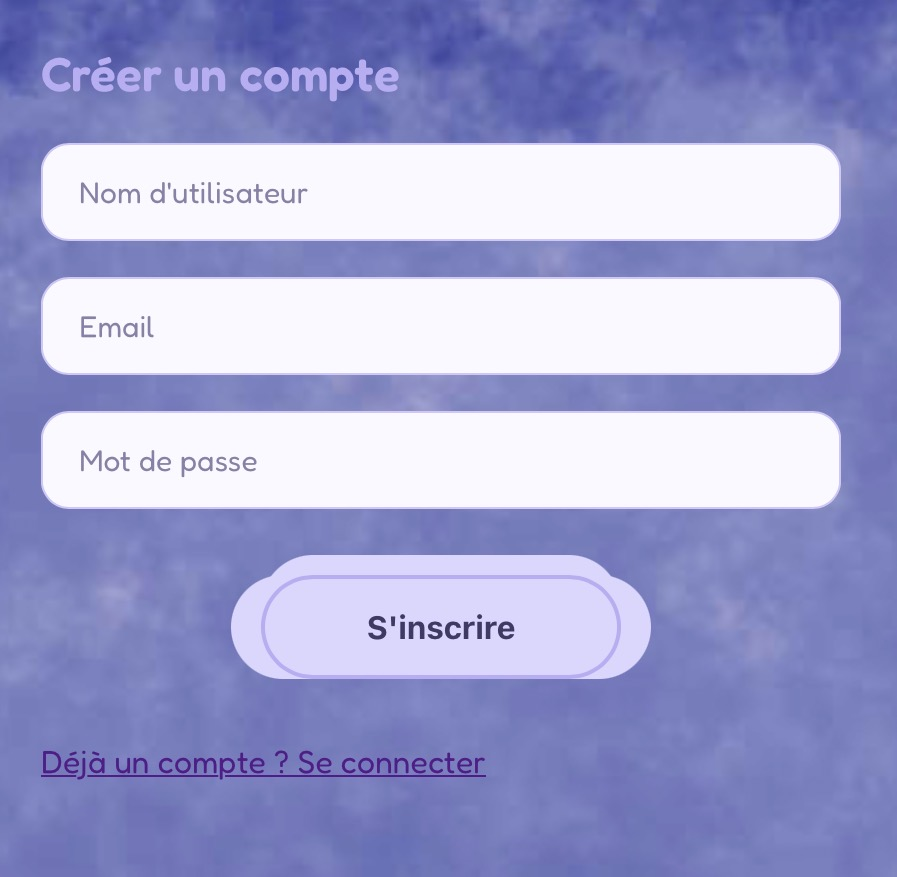
\includegraphics[width=0.5\textwidth]{crea}
\caption{Création d'un compte}
\label{fig:structure}
\end{figure}

Page de connexion : 
\begin{figure}[!ht]
\centering
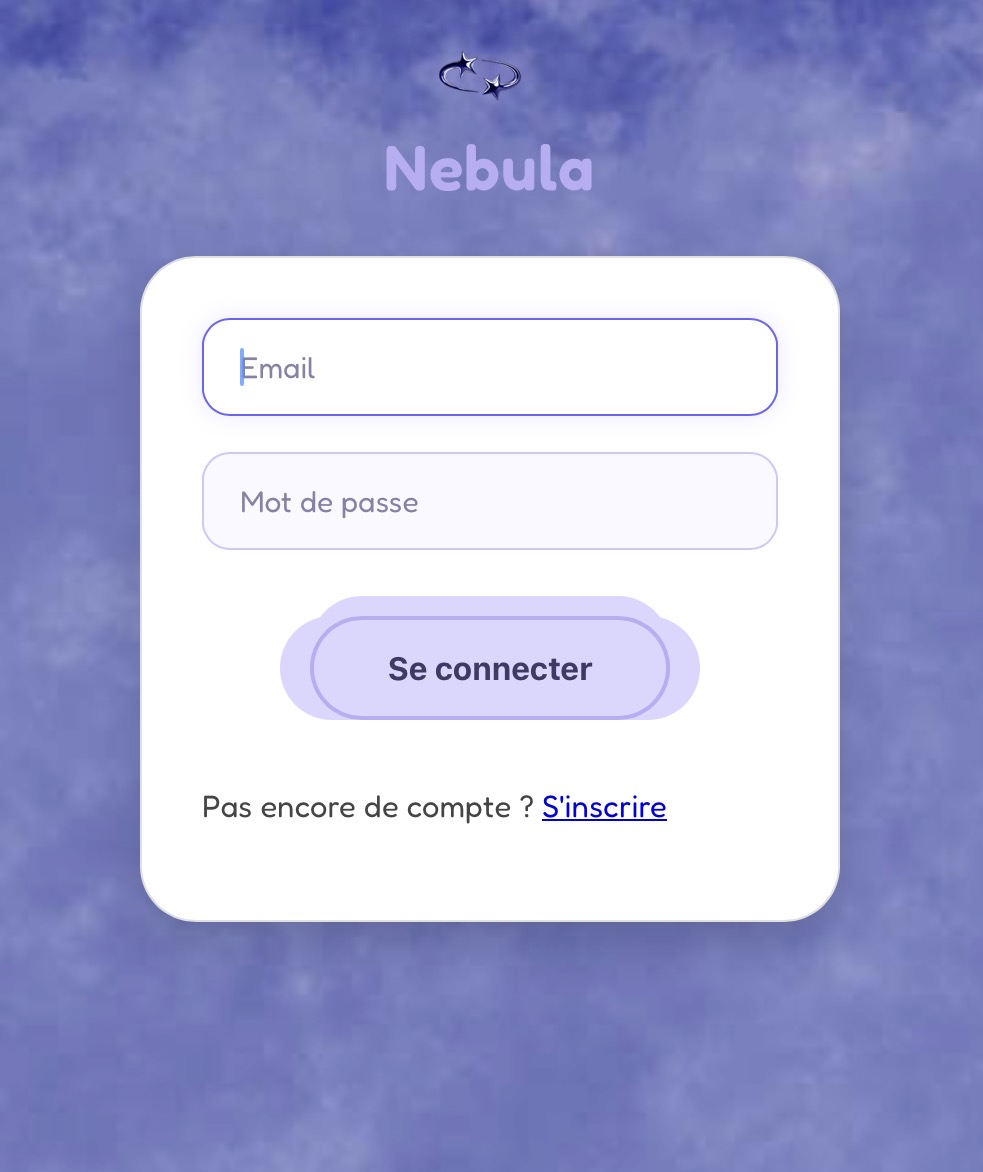
\includegraphics[width=0.5\textwidth]{cnx}
\caption{Connexion au compte}
\label{fig:structure}
\end{figure}\\
\newpage
Tableau de bord (Profil) :
\begin{figure}[!ht]
\centering
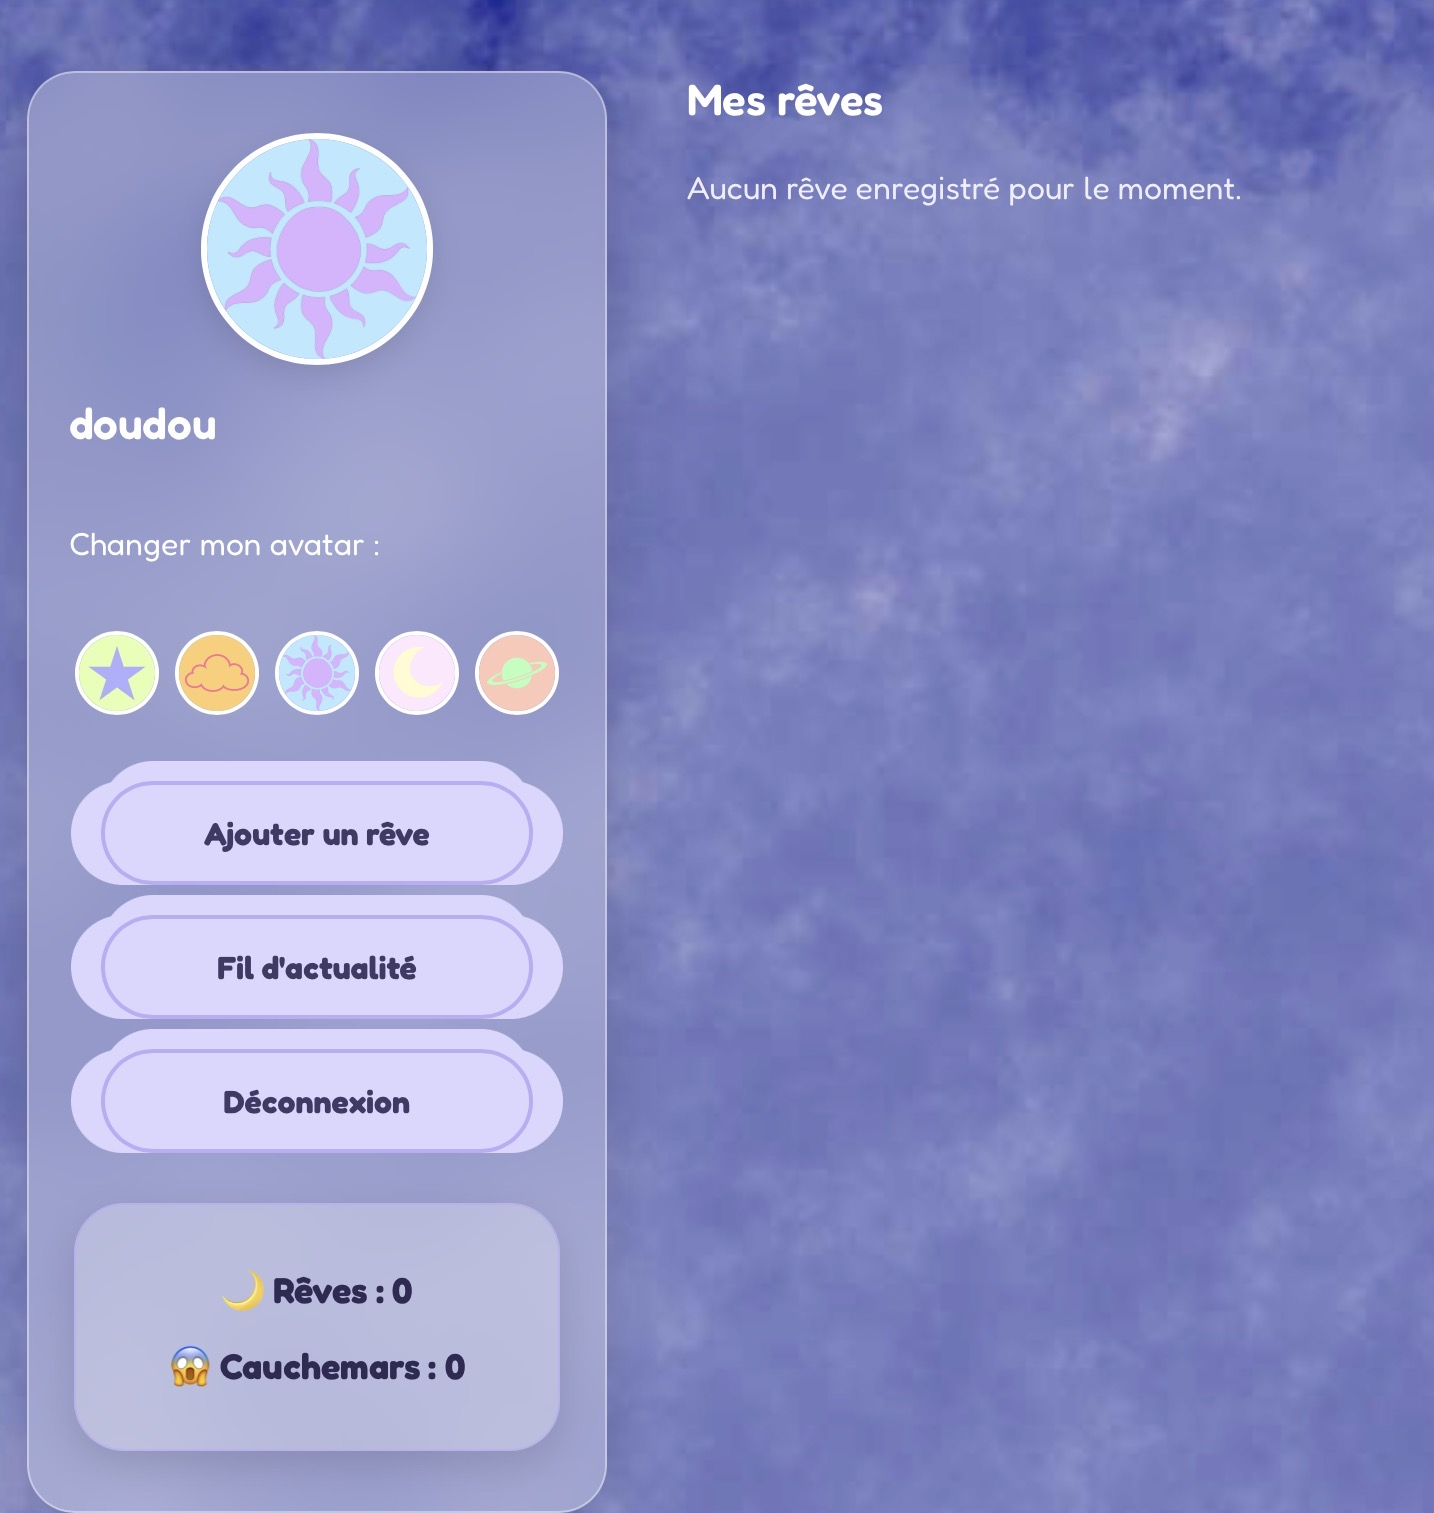
\includegraphics[width=0.5\textwidth]{Profil}
\caption{Tableau de bord}
\label{fig:structure}
\end{figure} \\
Exemple du feed (fil d'actualité):
\begin{figure}[!ht]
\centering
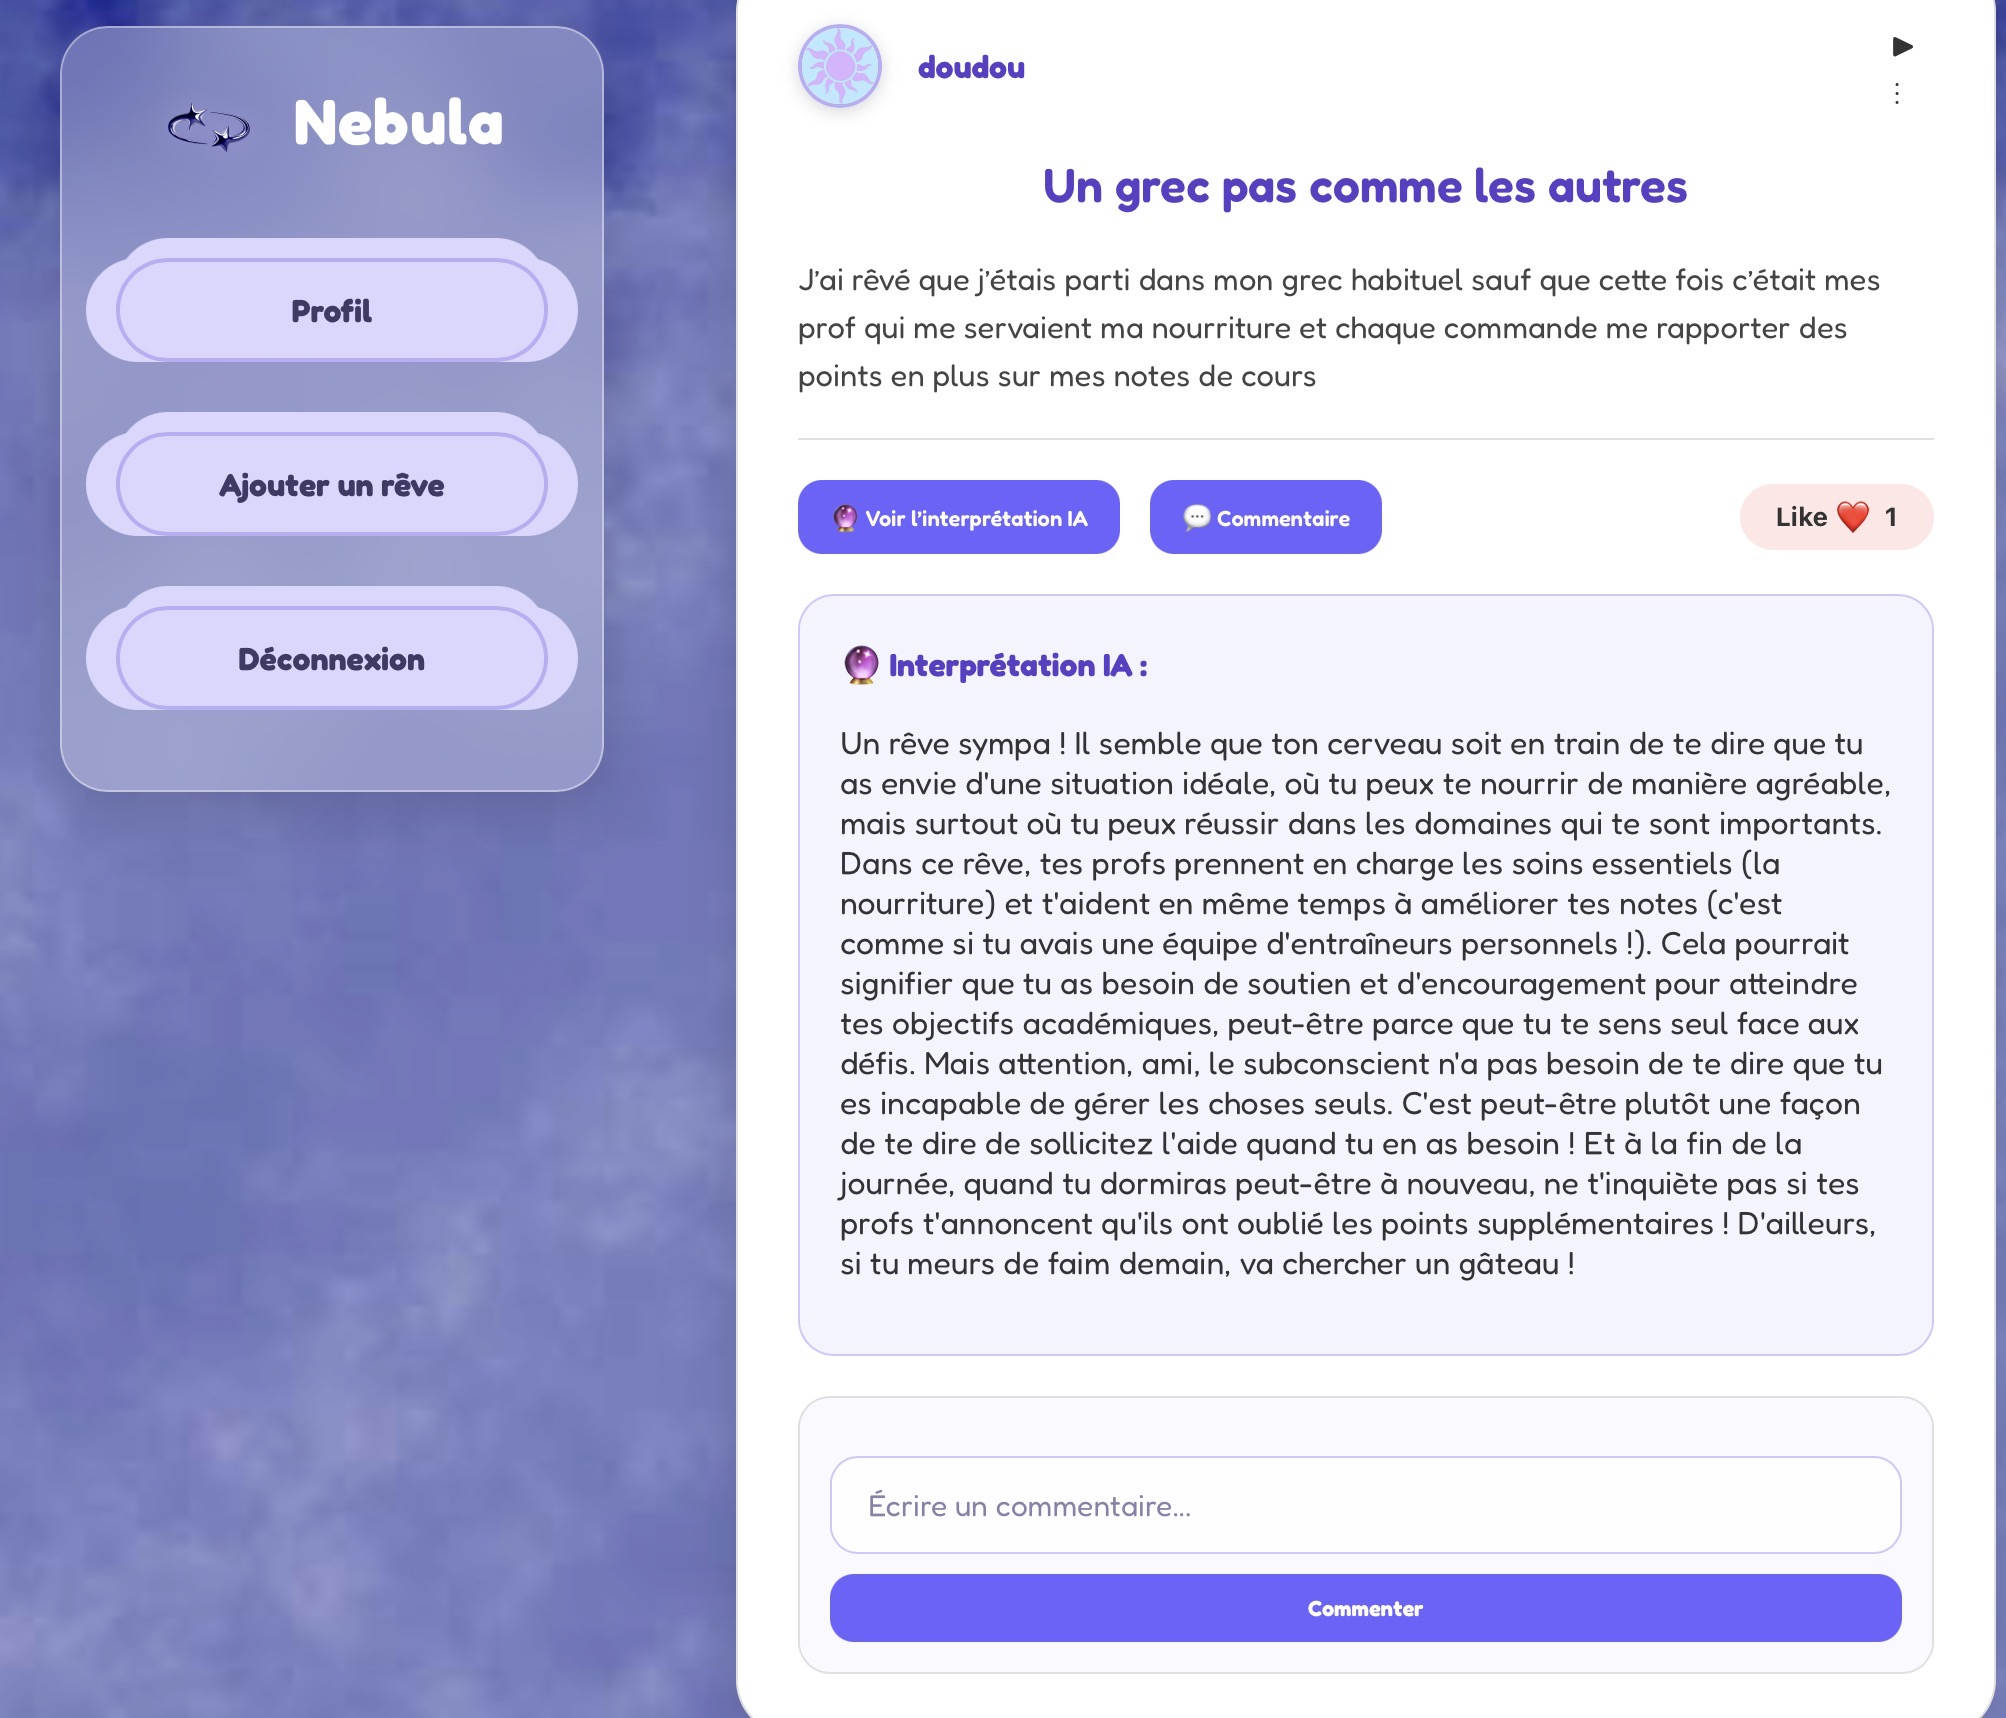
\includegraphics[width=0.5\textwidth]{feed}
\caption{Fil d'actualité}
\label{fig:structure}
\end{figure} \\

\newpage
	\section{Manuel utilisateur}

1) En entrant sur le site, cliquer sur le bouton ”S'inscrire”, en dessous du bouon "Se connecter"\\
2) Création d’un compte - attention à ne pas utiliser unmail déjà pris, sinon, la page de connexion rechargera\\
3) Redirection vers la page de connexion - taper son mail et mot de passe à l’identique\\
4) Arrivée sur le Feed cliquer sur "Ajouter un rêve"\\
5) Écrirez votre rêve ou cauchemar et choissiez de le publier ou non\\ 
6) Vous êtes redirigé vers le Tableau de bord : vous pouvez voir toutes vos publications\\
7) À vous maintenant de découvrir le site à travers les publications de chacun \\

\end{document}